\documentclass{article}
\usepackage{amsmath}
\usepackage{amssymb}
\usepackage{ctex}
\usepackage[margin=2cm]{geometry} % 设置较窄的边距使文档宽一些
\usepackage{multirow} % 支持表格中的多行单元格
\usepackage{graphicx} % 用于插入图片
\usepackage{float}
\title{\heiti\zihao{2} 金属冲击试验}
\author{\songti author  Student ID  }
\date{2024.5.20}
\begin{document}
    \maketitle

\begin{abstract}
    我们通过实验,分别测得低碳钢和铸铁的冲击韧性值 $\alpha_{\mathrm{k}}$ ,比较两种材料的抗冲击能力和断口形貌。实验中我们使用了冲击试验机,采用常温、简支梁式、大能量一次性冲击试验。实验结果表明,低碳钢的冲击韧性值大于铸铁的冲击韧性值,说明低碳钢的抗冲击能力更强。

    \noindent{\textbf{关键词:} 冲击载荷;冲击试验;冲击韧性}
    
\end{abstract}
\section{引言}
冲击载荷是指载荷在与承载构件接触的瞬时内速度发生急剧变化的情况。气
动凿岩机械、锻造机械等所承受的载荷即为冲击载荷。 
冲击载荷作用下,若材料尚处于弹性阶段,其力学性能与静载下基本相同。
例如在这种情况下,钢材的弹性模量 E 和泊松比μ等都无明显变化。但在冲击载
荷作用下材料进入塑性阶段后,其力学性能却与静载下的有显著不同,例如塑性
性能良好的材料,在冲击载荷作用下,会呈现脆化倾向,发生突然断裂。由于冲
击问题的理论分析较为复杂,因而在工程实际中经常以实验手段检验材料的抗冲
击性能。 
冲击试验的分类方法较多,从温度上分有高温、常温、低温三种;从受力形
式上分包括拉伸冲击、扭转冲击和弯曲冲击等,弯曲冲击较易获得脆断现象,并
且方法简单,因此得到广泛应用。


\section{实验目的}
\begin{enumerate}
    \item 了解冲击韧性的含义 
    \item 测定低碳钢和铸铁的冲击韧性值 $\alpha_{\mathrm{k}}$ ,比较两种材料的抗冲击能力和断口形貌
\end{enumerate}

\section{实验器材}

冲击试验机
 
\section{冲击试样}
工程上常用的金属材料冲击试样一般为带缺口矩形试样,冲击韧性 $A_k$ 的值
与试样的尺寸、缺口形状和支承方式有关。为便于比较,国家标准规定两种形式
的试样:   
    \begin{enumerate}
        \item U 形缺口试样
        \item V 形缺口试样
    \end{enumerate} 

\begin{figure}[h]
    \centering
    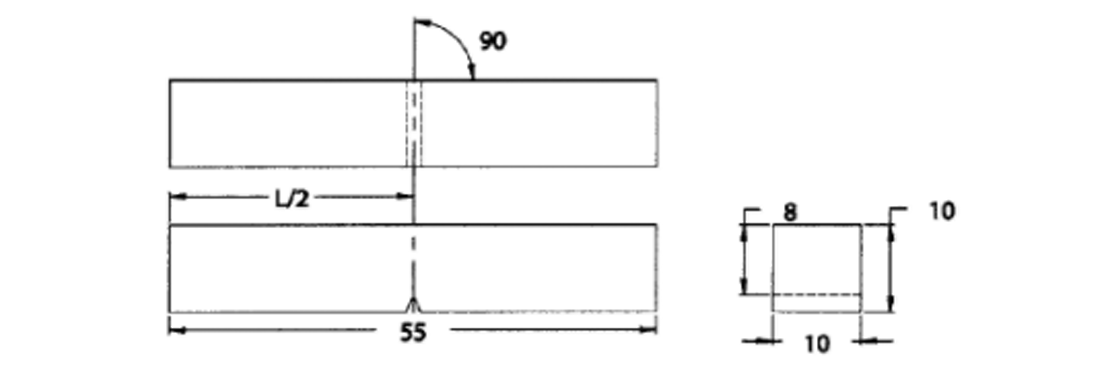
\includegraphics[width=0.8\textwidth]{img1.png}
    \caption{试样尺寸}
    \label{fig:diff_circuit}
\end{figure}

\section{实验原理}
材料在冲击载荷作用下,产生弹、塑性变形和断裂过程中吸收能量的能力,
定义为材料的冲击韧性。用实验方法测定材料的冲击韧性时,是把材料制成标准
试样,置于能实施打击能量的冲击试验机上进行的,并用折断试样的冲击吸收功
来衡量。

1) 冲击实验是研究材料对于动载荷抗力的一种实验,和静载荷作用不同,
由于加载速度快,使材料内的应力骤然提高,变形速度影响了材料的机构性质,
所以材料对动载荷作用表现出另一种反应。往往在静载荷下具有很好塑性性能的
材料,在冲击载荷下会呈现出脆性的性质。

2) 此外在金属材料的冲击实验中,还可以揭示静载荷时,不易发现的结构
特点和工作条件对机械性能的影响(如应力集中,材料内部缺陷,化学成分和加
载时温度、受力状态以及热处理情况等),因此它在工艺分析比较和科学研究中
都具有一定的意义 

3) 本试验采用的常温、简支梁式、大能量一次性冲击试验,依据是国家标
准 GB/T229-2007《金属材料 夏比摆锤冲击试验方法》

冲击试验机由摆锤、机身、支座、度盘、指针等几部分组成。实验时,将带有缺口的试样安放于试验机的支座上,举起摆锤使它自由下落将试样冲断。若摆锤重量为 G,冲击中摆锤的质心高度由 $H_1$ 变为 $H_2$ ,势能的变化为 $G\left(H_1-H_2\right)$ ,它等于冲断试样所消耗的功 $W$ ,亦即冲击中试样所吸收的功为

$$
A_K=W=G\left(H_1-H_2\right)
$$

$A_K$ 值越大,表明材料抗冲击性能越好。 $A_K$ 是一个综合性的参数,不能直接用于设计,但可作为抗冲击构件选择材料的重要指标。

冲击过程所消耗的能量,除大部分被试样断裂所吸收外,还有一小部分消耗于机座振动等方面。

\begin{figure}[H]
    \centering
    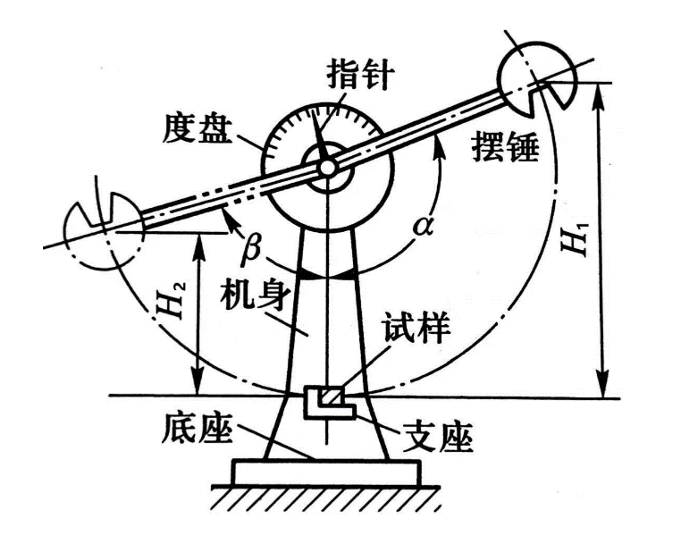
\includegraphics[width=0.6\textwidth]{img2.png}
    \caption{冲击装置示意图}
    \label{fig:diff_circuit}
\end{figure}
\begin{figure}[H]
    \centering
    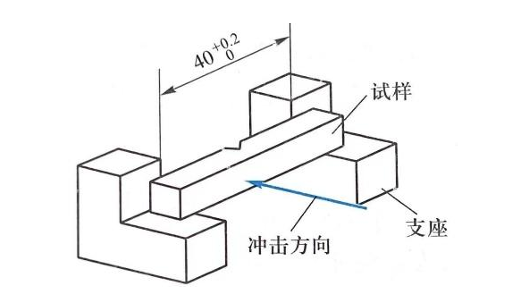
\includegraphics[width=0.6\textwidth]{img3.png}
    \caption{试样放置示意图}
    \label{fig:diff_circuit}
\end{figure}

\section{实验方法与步骤}

(1)了解摆锤冲击试验机的构造原理和操作方法,掌握冲击试验机的操作规程,一定要注意安全。

(2)空打试验。举摆,不放试样,空打一次,记录

(3)用取样钳将试件放在在冲击试验机的砧座上,简支梁式冲击实验应使没有缺口的面朝向摆锤冲击的一边,缺口的位置应在两支座中间,要使缺口和摆锤刀刃对准。将摆锤举起,按下"冲击",摆锤落下,冲断试样,读出试样冲断时消耗的功 $W$ ,用下式计算出材料的冲击韧性 $\alpha_{\mathrm{k}}$

$$
\alpha_{\mathrm{k}}=\frac{W}{A}
$$


W——冲断试件时所消耗的功 

A——试件缺口横截面积 

\section{实验数据处理}
\begin{figure}[H]
    \centering
    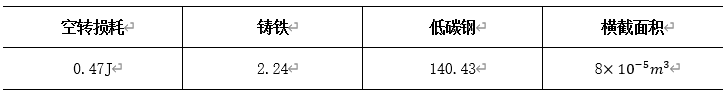
\includegraphics[width=0.8\textwidth]{img4.png}
    \caption{实验数据}
    \label{fig:diff_circuit}
\end{figure}

铸铁的冲击韧性 
$$
\alpha_{\mathrm{k}}=\frac{2.24-0.47}{8\times {10}^{-5}}=2.2125\times {10}^{4}J/m^3
$$

低碳钢的冲击韧性 
$$
\alpha_{\mathrm{k}}=\frac{140.43-0.47}{8\times {10}^{-5}}=1.7495\times {10}^{6}J/m^3
$$

\section{参考文献}
[1] 金属材料拉伸试验。实验讲义.


% \newpage
% 需要指出:由于 GB/T 10128-2007 在计算屈服极限 $\tau_s$ 和抗扭强度 $\tau_b$ 时,仍是以切应力线性分布为依据,即

% $$
% \tau_s=\frac{T_s}{W}
% $$


% 而试样横截面上的切应力的真实分布为均匀分布,真实屈服极限应该按下式计算:
% $$
% \tau_{\text {strue }}=\frac{3}{4} \frac{T_s}{W}
% $$


% 由上两式可知,$\tau_{\text {strue }}$ 比 $\tau_s$ 要小一些,真实屈服极限 $\tau_{\text {strue }}$ 约为屈服极限 $\tau_s$ 的 $75 \%$ ,推导公式如下:

% 在达到 $T_s$ 时,假定截面上各点的剪应力同时达到屈服极限 $\tau_{\mathrm{S}}$(理想塑性),断面上 $\tau_{\mathrm{s}}$ 均匀分布,从而推导计算屈服极限的近似公式如下:

% 因

% $$
% T_s=\int_F\left(\tau_s d A\right) \cdot \rho
% $$


% 式中 $\tau_{\mathrm{s}}$ 是常数,

% $$
% \mathrm{d} A=2 \pi \rho \cdot \mathrm{~d} \rho
% $$


% 所以

% $$
% T_s=\tau_s \int_0^R \rho \cdot 2 \pi \rho \cdot d \rho=2 \pi \tau_s \int_0^R \rho^2 d \rho
% $$

% 所以

% $$
% T_s=\tau_s \int_0^R \rho \cdot 2 \pi \rho \cdot d \rho=2 \pi \tau_s \int_0^R \rho^2 d \rho=\frac{2 \pi R^3}{3} \cdot \tau_{\mathrm{s}}=\frac{4}{3} \cdot \frac{\pi R^3}{2} \cdot \tau_{\mathrm{s}}=\frac{4}{3} W_{\mathrm{p}} \tau_{\mathrm{s}}
% $$

% 故屈服极限 

% $$\quad \tau_s=\frac{3 T_s}{4 W_p}$$


% 式中:$W_p=\frac{\pi}{16} d^3=\frac{\pi}{2} R^3$

% 与屈服时的塑性变形过程相似,可得抗扭强度 
% $$
% \tau_b=\frac{3 T_b}{4 W_p}
% $$




\end{document}